% This is auto-generated file: do not edit!
% Exported from microMathematics Plus, version 2.20.0


Esta app es un potente software de
cálculo en formato de hoja de cálculo.
La hoja de cálculo puede ser editada
libremente, almacenada
 o abierta en una tarjeta SD, y
exportada a una imagen o formato
LaTeX.

La hoja de cálculo es un documento
matemático que contiene texto,
fórmulas y gráficos. Soporta la
edición en vivo de notaciones
matemáticas y su cálculo automático.

Los siguientes objetos pueden ser
insertados en hoja de trabajo:
ecuaciones, vistas de resultados,
gráficos, fragmentos de texto e
imágenes. Este documento da una visión
general de cómo editar estos objetos.

\subsection{Edición}

Casi todos los objetos disponibles
contienen varios campos editables.
Para editar el campo use los símbolos
y funciones en la barra de
herramientas.

Todos los símbolos también pueden ser
introducidos desde el teclado. Para
saber cuál símbolo del teclado
corresponde al símbolo matemático que
desea introducir, lea la pista al
mantener presionado en el botón de
interés.

Con un clic largo en un término puede
seleccionar este término. El término
seleccionado puede borrarse, copiarse
al portapapeles, pegarse desde este
elemento o puede insertar otro
operador u otra función después de ese
término utilizando los botones de la
barra de herramientas o del teclado.

El comando ''Deshacer'' está disponible
en la barra de acción. Borra el último
cambio realizado en el documento y lo
devuelve a un estado anterior:
\begin{center}\begin{tabular}{c} 
\includegraphics[width=0.45\textwidth]{graphics/how_to_use_fig1.png} \end{tabular}\end{center}

\subsection{Ecucación}

Una ecuación define una constante
numérica, un intervalo o una función.
Para crear una ecuación, use el botón
''Nuevo elemento'' en la barra de
acciones
\begin{center}\begin{tabular}{c} 
\includegraphics[width=0.45\textwidth]{graphics/how_to_use_fig2.png} \end{tabular}\end{center}

o el botón ''Añadir ecuación'' de la
barra de herramientas:
\begin{center}\begin{tabular}{c} 
\includegraphics[width=0.45\textwidth]{graphics/how_to_use_fig3.png} \end{tabular}\end{center}

Aparece una ecuación con dos campos
vacíos. Estos campos deben ser
rellenados:
\begin{center}\begin{tabular}{c}
  ${\Box} := {\Box}$
\end{tabular}\end{center}

El nombre de la ecuación se da en el
campo de la izquierda. El nombre debe
llevar únicamente letras o dígitos y
se utilizará en otros objetos para
hacer referencia a esta ecuación.

Desde la barra de acciones, puede
abrir la ventana de diálogo ''Ajustes
del documento'': 
\begin{center}\begin{tabular}{c} 
\includegraphics[width=0.45\textwidth]{graphics/how_to_use_fig4.png} \end{tabular}\end{center}

Dependiendo del parámetro ''Permitir 
redefinición de ecuaciones'' en este
diálogo, hay dos modos de uso: 

a) si no se permite la redefinición,
el nombre de la ecuación será único
dentro de toda la hoja de trabajo y la
ecuación puede utilizarse tanto antes
como después de su definición,

b) si se permite la redefinición,
puedes definir más de una ecuación con
el mismo nombre. Si tal ecuación está
referenciada, la última versión
definida antes de la ecuación llamada
será utilizada.

\subsubsection{Constant}

Si el nombre de la ecuación no contiene
algún argumento entre paréntesis, se
define una constante o un intervalo:
\begin{center}\begin{tabular}{ccc}
  $N := 200$ &
  $Sq2 := \sqrt{100} $ &
  $Pi2 := \frac{{\pi}}{2}$ \cr
\end{tabular}\end{center}

En el último ejemplo, se usó una
constante pi preparada. Actualmente,
las siguientes constantes incorporadas
están disponibles:
\begin{center}\begin{tabular}{ccc}
  ${\pi} = 3.14159$ &
  $pi = 3.14159$ &
  $e = 2.71828$ \cr
\end{tabular}\end{center}

Una constante previamente definida
también puede  ser usada:
\begin{center}\begin{tabular}{c}
  $NPi2 := N \cdot Pi2$
\end{tabular}\end{center}

También puede utilizar el símbolo ''i''
como unidad imaginaria para definir un
número complejo:
\begin{center}\begin{tabular}{c}
  $z := 5+3i$
\end{tabular}\end{center}

\subsubsection{Units}

Si necesitas una unidad para la
constante, puedes ponerla desde el
teclado en el mismo campo de entrada.
La unidad deberá estar separada del
número usando espacio. Puedes usar
unidades tanto para las constantes
reales, como para las complejas:
\begin{center}\begin{tabular}{ccc}
  $r := 10 m$ &
  $a := {10 m}^{2}$ &
  $v := 10 km / hr$ \cr
\end{tabular}\end{center}
\begin{center}\begin{tabular}{cc}
  ${\alpha} := 45 {\degree} + 30 ' + 15 ''$ &
  ${\varphi} := 100 \cdot \frac{kg \cdot m}{{s}^{2}}$ \cr
\end{tabular}\end{center}

El documento ''units\_overview.mmt''
contiene la lista de todas las
unidades soportadas . Este documento
se entrega con la aplicación y se
almacena en ''Recursos de
microMathematics Plus''.

\subsubsection{Interval}

Una ecuación de tipo intervalo define
una variable que se cambia desde un
valor mínimo hasta un valor máximo
dado con un incremento definido. Esta
variable puede ser utilizada como
argumento para gráficos de función o
como parámetro para elaborar una tabla
de valores de función.

Para definir un intervalo, ponga un
nombre válido a la izquierda de una
ecuación vacía. En el lado derecho de
esta ecuación, ponga un símbolo '':'', o
pulse en el botón ''Intervalo
equidistante'' de la barra de
herramientas:
\begin{center}\begin{tabular}{c} 
\includegraphics[width=0.45\textwidth]{graphics/how_to_use_fig5.png} \end{tabular}\end{center}

Aquí, el primer elemento es el
intervalo como punto de inicio, el
siguiente elemento es el segundo
punto, y el último elemento es el
punto final del intervalo:
\begin{center}\begin{tabular}{c}
  $x := \left[ 0,\, 0.1 \,..\, 10 \right]$
\end{tabular}\end{center}

Se accederá a los elementos del
intervalo por índice:
\begin{center}\begin{tabular}{ccc}
  $x_{0}  = 0.0$ &
  $x_{1}  = 0.1$ &
  $x_{100}  = 10.0$ \cr
\end{tabular}\end{center}

El incremento es la diferencia de dos
valores vecinos:
\begin{center}\begin{tabular}{c}
  $x_{2}  - x_{1}  = 0.1$
\end{tabular}\end{center}

Por ejemplo, podemos definir un
intervalo equidistante que contiene N
puntos distribuidos con el incremento
''dy'' donde el inicio del intervalo es
cero como sigue:
\begin{center}\begin{tabular}{cc}
  $dy := 0.05$ &
  $y := \left[ 0,\, dy \,..\, dy \cdot N \right]$ \cr
\end{tabular}\end{center}

\subsubsection{Function}

Una función es una relación entre uno o
más argumentos y un conjunto de
salidas permisibles con la propiedad,
que cada valor del argumento (real o
complejo) o combinación de argumentos
está relacionado exactamente con la
salida.

El nombre de la función el argumento
de la función entre paréntesis se dan
en el lado izquierdo de una ecuación.
No es necesario definir el argumento
en la hoja de trabajo previamente,
puedes definirlo como quieras, pero
usando sólo letras o dígitos:
\begin{center}\begin{tabular}{c}
  $f(t) := sin \left( t\right)  \cdot cos \left( t\right)  / 2$
\end{tabular}\end{center}
\begin{center}\begin{tabular}{c}
  $w(z) := {e}^{2i \cdot {\pi} \cdot z}$
\end{tabular}\end{center}
\begin{center}\begin{tabular}{c}
  $H(x,y) := \sqrt{{x}^{2} + {y}^{2}} $
\end{tabular}\end{center}
\begin{center}\begin{tabular}{c}
  $g(x,y) := \frac{sin \left( H \left( x,\, y\right) \right) }{H \left( x,\, y / 2\right)  + 1}$
\end{tabular}\end{center}

El lado derecho de la función contiene
una fórmula matemática de cómo
calcular la función. Si esta fórmula
no contiene el argumento declarado en
la función, tal función se
interpretará como una constante.

También puedes utilizar en el lado
derecho otras funciones incorporadas o
previamente definidas . Para insertar
una función introduzca su nombre,
pulse en el corchete izquierdo el
símbolo ''('' y luego introduzca su
argumento. Este argumento también
puede ser un fórmula, que contiene
cualquier otra operación y función.

El documento ''functions\_overview.mmt'',
almacenado dentro de los ''Recursos de
microMathematic Plus'', proporciona la
lista de todas las funciones
disponibles.

\subsubsection{Matriz}

Las matrices son funciones especiales
con las siguientes propiedades:

a) los elementos de la matriz pueden
asignarse usando un índice dado en [ ]
en lugar de ( ). Cualquier elemento no
asignado es  establecido por defecto a
cero:
\begin{center}\begin{tabular}{ccc}
  $r[0] := 5$ &
  $r[3] := 6$ &
  $r[2] := -4$ \cr
\end{tabular}\end{center}
\begin{center}\begin{tabular}{cc}
  $idx := \left[ 0,\, 1 \,..\, 3 \right]$ &
  $r_{idx}  = \begin{bmatrix}5.0\\0.0\\-4.0\\6.0\\\end{bmatrix}$ \cr
\end{tabular}\end{center}

b) un intervalo previamente definido
puede ser usado como argumento de la
matriz:
\begin{center}\begin{tabular}{cc}
  $k := \left[ 0,\, 1 \,..\, 100 \right]$ &
  $m := \left[ 0,\, 1 \,..\, 200 \right]$ \cr
\end{tabular}\end{center}
\begin{center}\begin{tabular}{c}
  $M[k,m] := {sin \left( k / 10\right) }^{2} - 3 \cdot  \left| cos \left( m / 10\right)  \right| $
\end{tabular}\end{center}

c) los elementos de la matriz se
calculan y se guardan en una memoria
que reduce el tiempo de acceso a estos
valores

d) sólo se puede acceder a los
elementos de la matriz utilizando un
índice inferior. Para crear un índice
inferior, ponga ''['' después del nombre
de la matriz:
\begin{center}\begin{tabular}{cc}
  $M_{5,\, 10}  = -1.39106$ &
  $M_{10,\, 5}  = -1.92467$ \cr
\end{tabular}\end{center}
\begin{center}\begin{tabular}{c}
  $P[k,m] := floor \left( -10 \cdot M_{k,\, m} \right) $
\end{tabular}\end{center}

e) si algún índice de la matriz es
complejo o negativo o mayor que el
límite superior del intervalo
correspondiente, se devolverá el
número inválido:
\begin{center}\begin{tabular}{cc}
  $M_{10i,\, 100}  = NaN$ &
  $M_{90,\, 210}  = NaN$ \cr
\end{tabular}\end{center}

\subsection{Result View}

Este elemento tiene como objetivo
representar un resultado de cálculo
como un número o una tabla. Para
añadir este elemento, utilice el botón
''Nuevo elemento'' de la barra de
acciones o el botón ''Añadir vista de
resultados'' de la barra de
herramientas:
\begin{center}\begin{tabular}{c} 
\includegraphics[width=0.45\textwidth]{graphics/how_to_use_fig6.png} \end{tabular}\end{center}

Aparece una ecuación con dos campos,
donde se rellenará el campo izquierdo:
\begin{center}\begin{tabular}{c}
  ${\Box} = {\Box}$
\end{tabular}\end{center}

El término de la izquierda contiene una
fórmula para ser calculada y el
término de la derecha es el resultado
del cálculo. El resultado se mostrará
cuando se presiona el botón flotante
''Calcular''.

Dentro del término de la izquierda se
puede utilizar cualquier constante y
funciones definidas previamente así
como cualquier función preparada:
\begin{center}\begin{tabular}{c}
  ${e}^{{\pi}} \cdot f \left( NPi2\right)  = 2.27286E-14$
\end{tabular}\end{center}

Si la parte izquierda no contiene
ninguna variable de ''tipo intervalo'',
el resultado del cálculo es sólo un
número real o complejo:
\begin{center}\begin{tabular}{c}
  $y_{N - 1}  - y_{0}  = 9.95$
\end{tabular}\end{center}
\begin{center}\begin{tabular}{ccc}
  $\Re\left( z \right)  = 5.0$ &
  $\Im\left( z \right)  = 3.0$ &
  $ \left| z \right|  = 5.83095$ \cr
\end{tabular}\end{center}
\begin{center}\begin{tabular}{c}
  $\sqrt{sin \left( \frac{3}{2} \cdot {\pi}\right) }  = 0.0+1.0i$
\end{tabular}\end{center}

Si la parte izquierda contiene alguna
variable que tenga una unidad
dimensional, entonces el resultado
puede tener dimensión también:
\begin{center}\begin{tabular}{c}
  $2 \cdot {\alpha} / 10 s = 0.15884 rad/s$
\end{tabular}\end{center}

Si la parte izquierda contiene un
intervalo variable, el resultado del
cálculo es un vector de valores
correspondiente a este intervalo.
Debido al límite de espacio libre en
la visualización, sólo se mostrarán
los seis primeros y los últimos
elementos del vector:
\begin{center}\begin{tabular}{ccc}
  $x = \begin{bmatrix}0.0\\0.1\\0.2\\0.3\\0.4\\0.5\\\dots\\10.0\\\end{bmatrix}$ &
  $y = \begin{bmatrix}0.0\\0.05\\0.1\\0.15\\0.2\\0.25\\\dots\\10.0\\\end{bmatrix}$ &
  $2 \cdot y = \begin{bmatrix}0.0\\0.1\\0.2\\0.3\\0.4\\0.5\\\dots\\20.0\\\end{bmatrix}$ \cr
\end{tabular}\end{center}
\begin{center}\begin{tabular}{c}
  $P_{k,\, m}  = \begin{bmatrix}30.0&29.0&29.0&28.0&\dots&12.0\\29.0&29.0&29.0&28.0&\dots&12.0\\29.0&29.0&29.0&28.0&\dots&11.0\\29.0&28.0&28.0&27.0&\dots&11.0\\\dots&\dots&\dots&\dots&\dots&\dots\\27.0&26.0&26.0&25.0&\dots&9.0\\\end{bmatrix}$
\end{tabular}\end{center}

El número de elementos visualizados y
el modo en el que se muestra el
resultado puede ser cambiado. Al
mantener presionado en el área de la
fórmula y el menú contextual
seleccione toda la fórmula. Si se
selecciona la fórmula, aparece el
botón flotante de ''Propiedades del
objeto''. Si se hace clic en este
botón, se mostrará el diálogo de vista
de resultados:
\begin{center}\begin{tabular}{c} 
\includegraphics[width=0.45\textwidth]{graphics/how_to_use_fig7.png} \end{tabular}\end{center}

El segundo botón flotante, ''Detalles'',
también aparecerá. Si hace clic en
este botón, se mostrará el diálogo
''Detalles'', donde podrá observar todos
los elementos de la matriz.

Observe que el uso de tres o más
variables ''tipo intervalo'' a la
izquierda parte de una vista de
resultados no está permitido en esta
versión de la aplicación.

\subsection{Gráfico de Funciones}

El elemento de la gráfica de la función
muestra una representación visual de
una función, que depende de un solo
argumento. Para crear un gráfico,
utilice el botón ''Nuevo elemento'' de
la barra de acciones o el botón
''Añadir gráfico de funciones'' de la
barra de herramientas:
\begin{center}\begin{tabular}{c} 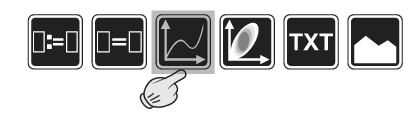
\includegraphics[width=0.45\textwidth]{graphics/how_to_use_fig8.png} \end{tabular}\end{center}

Aparece un panel con seis campos
vacíos. La función que se va a
graficar deberá ser puesta en el campo
medio-izquierdo y el argumento de la
función en el campo medio-inferior:
\begin{center}\begin{tabular}{c} 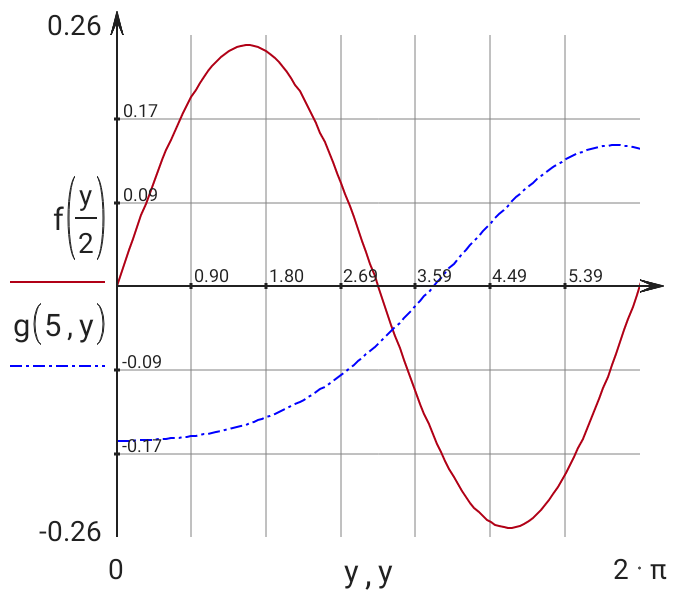
\includegraphics[width=0.45\textwidth]{graphics/how_to_use_fig9.png} \end{tabular}\end{center}

Para más detalles ver ''Gráfica de
funciones'' y ejemplos de ''Gráfica de
funciones polares'' del cajón de
navegación de aplicaciones.

\subsection{Gráfica tridimensional}

El elemento de la gráfica 3D muestra un
gráfico de una sola función que
depende de dos argumentos. Para crear
un gráfico de este tipo, utilice el
botón ''Nuevo elemento'' de la barra de
acciones o el botón ''Añadir gráfico
3D'' de la barra de herramientas:
\begin{center}\begin{tabular}{c} 
\includegraphics[width=0.45\textwidth]{graphics/how_to_use_fig10.png} \end{tabular}\end{center}
\begin{center}\begin{tabular}{cc}
  $x := \left[ -10,\, -9.5 \,..\, 10 \right]$ &
  $y := \left[ -10,\, -9.5 \,..\, 10 \right]$ \cr
\end{tabular}\end{center}
\begin{center}\begin{tabular}{c} 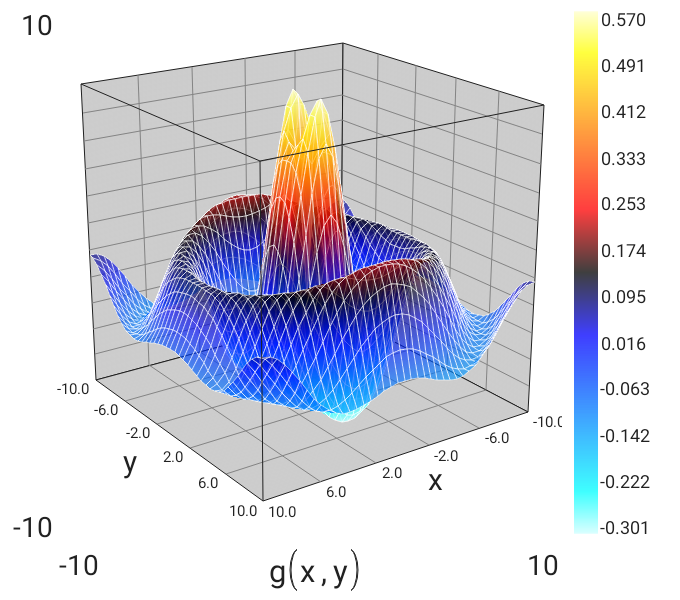
\includegraphics[width=0.45\textwidth]{graphics/how_to_use_fig11.png} \end{tabular}\end{center}

En el campo central-inferior, coloca el
nombre de la función o una ecuación
que contiene exactamente dos
intervalos previamente definidos. El
uso de una matriz también es posible:
\begin{center}\begin{tabular}{c} 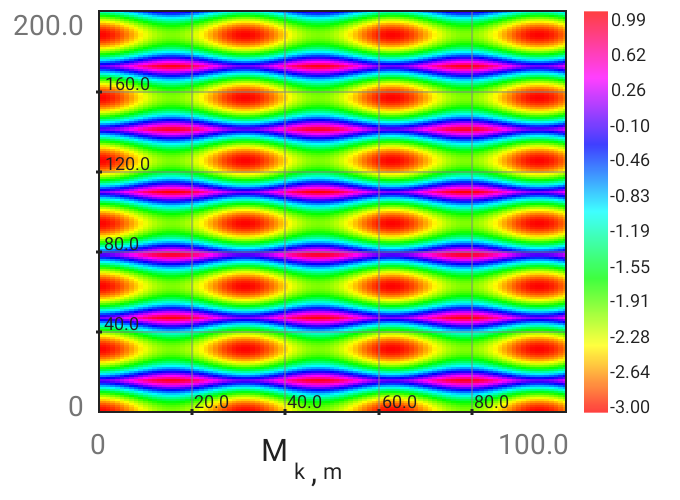
\includegraphics[width=0.45\textwidth]{graphics/how_to_use_fig12.png} \end{tabular}\end{center}

Para más detalles vea el ejemplo
''Gráfico 3D'' del cajón de navegación
de aplicaciones.

\subsection{Fragmento de texto}

El elemento de fragmento de texto
muestra un texto simple como este.
Para añadir un fragmento de texto,
utilice el botón ''Nuevo elemento'' de
la barra de acciones o el botón
''Añadir fragmento de texto'' de la
barra de herramientas:
\begin{center}\begin{tabular}{c} 
\includegraphics[width=0.45\textwidth]{graphics/how_to_use_fig13.png} \end{tabular}\end{center}

Si todo el texto dentro de un fragmento
es  seleccionado mediante el menú
contextual ''Seleccionar todo'',
aparecerá un botón flotante
''Propiedades del objeto'' en la parte
inferior derecha de la pantalla.

Si pulsa en este botón, aparecerá el
diálogo ''Propiedades de texto'', donde
podrá seleccionar el estilo de texto y
activar la numeración. Por ejemplo,
los títulos de este documento tienen
el estilo ''Subsección'' con la
numeración activada.

\subsection{Image}

También puedes insertar una imagen del
archivo de imágenes. Para hacerlo, usa
el botón ''Nuevo elemento'' de la barra
de acciones o el botón ''Añadir imagen
desde archivo'' de la barra de
herramientas:
\begin{center}\begin{tabular}{c} 
\includegraphics[width=0.45\textwidth]{graphics/how_to_use_fig14.png} \end{tabular}\end{center}

Aparecerá el diálogo '' Ajustes de
imagen''. Allí puede seleccionar un
archivo con la imagen que se va a
insertar y establecer el tamaño de
imagen necesario.

Los siguientes formatos de imagen son
soportados: png, bmp, gif, jpeg, svg.

Si activa el indicador ''Imagen
incrustada'' en el diálogo ''Ajustes de
imagen'', entonces la imagen se
incrustará directamente en el
documento. La imagen incrustada
operará dentro del único documento,
excepto en un archivo más grande.

Si el indicador ''Imagen incrustada'' no
está activado, el archivo de imagen
sólo será referenciado en lugar de
incrustarlo, es decir, su documento
vinculará al archivo de la imagen por
separado. En caso de que mueva su
documento por favor no olvide mover el
archivo de imagen también.

Puede cambiar las propiedades de una
imagen ya existente. Mantén presionado
en el área de la imagen hasta que
aparezca el botón flotante de
''Propiedades del objeto''. Si presiona
este botón, se mostrará un diálogo con
las propiedades de la imagen.